% Practice Test 02 — Alaska Edition
% Questions: 30 (22 MC + 8 SA)
% Generated by scripts/generate_practice_tests.py

\begin{practiceQuestion}{1-3-q30}{gsa}
\begin{questionText}
The table shows a proportional relationship between minutes and laps completed. Find $k$ and determine how many laps are completed in $15$ minutes.

\begin{center}
\begin{tabular}{|c|c|}
\hline
\textbf{Minutes ($x$)} & \textbf{Laps ($y$)} \\ \hline
$4$ & $3$ \\ \hline
$8$ & $6$ \\ \hline
$12$ & $9$ \\ \hline
$15$ & $?$ \\ \hline
\end{tabular}
\end{center}
\end{questionText}
\correctAnswer{$k = 0.75$; $11.25$ laps in $15$ minutes}
\explanation{$k = \frac{3}{4} = 0.75$. For $15$ minutes: $y = 0.75 \times 15 = 11.25$ laps.}
\end{practiceQuestion}

\begin{practiceQuestion}{1-5-q07}{mc}
\begin{questionText}
A line passes through $(0, 0)$ and has a slope of $\frac{3}{4}$. What is the $y$-value when $x = 8$?
\end{questionText}
\choiceA{$3$}
\choiceB{$6$}
\choiceC{$8$}
\choiceD{$11$}
\correctAnswer{B}
\explanation{$y = \frac{3}{4} \times 8 = 6$.}
\end{practiceQuestion}

\begin{practiceQuestion}{1-6-q25}{sa}
\begin{questionText}
A truck delivers $540$ packages in $3$ trips. How many trips are needed to deliver $1{,}620$ packages?
\end{questionText}
\correctAnswer{$9$ trips}
\explanation{Per trip: $540 \div 3 = 180$ packages. Trips needed: $1{,}620 \div 180 = 9$.}
\end{practiceQuestion}

\begin{practiceQuestion}{2-2-q13}{mc}
\begin{questionText}
A town has $2{,}400$ households. A survey shows $78\%$ have internet access. How many households have internet?
\end{questionText}
\choiceA{$1{,}800$}
\choiceB{$1{,}848$}
\choiceC{$1{,}872$}
\choiceD{$1{,}920$}
\correctAnswer{C}
\explanation{$\frac{n}{2400} = \frac{78}{100}$. Cross-multiply: $100n = 187{,}200$. Divide: $n = 1{,}872$.}
\end{practiceQuestion}

\begin{practiceQuestion}{2-5-q06}{mc}
\begin{questionText}
A taxi ride costs $\$18$. You tip the driver $18\%$. What is the total you pay?
\end{questionText}
\choiceA{$\$3.24$}
\choiceB{$\$19.80$}
\choiceC{$\$21.24$}
\choiceD{$\$21.60$}
\correctAnswer{C}
\explanation{Tip: $18 \times 0.18 = \$3.24$. Total: $18 + 3.24 = \$21.24$.}
\end{practiceQuestion}

\begin{practiceQuestion}{3-1-q10}{mc}
\begin{questionText}
A football team gains $8$ yards on one play and loses $8$ yards on the next play. What is the net result?
\end{questionText}
\choiceA{$16$ yards gained}
\choiceB{$8$ yards gained}
\choiceC{$8$ yards lost}
\choiceD{$0$ yards}
\correctAnswer{D}
\explanation{$8 + (-8) = 0$. Gaining and losing the same amount are opposite actions that cancel out.}
\end{practiceQuestion}

\begin{practiceQuestion}{3-2-q30}{gsa}
\begin{questionText}
A thermometer shows temperature changes over three hours.

\begin{center}
\begin{tikzpicture}
  \draw[thick,->] (0,-4.5) -- (0,4.5);
  \foreach \y in {-4,...,4} \draw (-0.15,\y) -- (0.15,\y) node[right=4pt] {$\y°$C};
  \fill[funBlue] (0,-3) circle (4pt);
  \node[left=8pt] at (0,-3) {Start: $-3°$C};
  \draw[thick,->,funGreen] (-0.6,-3) -- (-0.6,1);
  \node[left] at (-0.6,-1) {\footnotesize $+4°$};
  \draw[thick,->,funRed] (-1.2,1) -- (-1.2,-2);
  \node[left] at (-1.2,-0.5) {\footnotesize $-3°$};
\end{tikzpicture}
\end{center}

What is the final temperature after these two changes?
\end{questionText}
\correctAnswer{$-2°$C}
\explanation{Start at $-3°$C. Rise $4°$: $-3 + 4 = 1°$C. Drop $3°$: $1 + (-3) = -2°$C.}
\end{practiceQuestion}

\begin{practiceQuestion}{3-3-q01}{mc}
\begin{questionText}
What is $10 - 16$?
\end{questionText}
\choiceA{$6$}
\choiceB{$-6$}
\choiceC{$26$}
\choiceD{$-26$}
\correctAnswer{B}
\explanation{Rewrite as $10 + (-16) = -6$. The larger absolute value ($16$) is negative.}
\end{practiceQuestion}

\begin{practiceQuestion}{3-10-q23}{sa}
\begin{questionText}
A submarine at $-300$ feet rises $\dfrac{3}{5}$ of the way to the surface. What is its new depth?
\end{questionText}
\correctAnswer{$-120$ feet}
\explanation{Rise: $\frac{3}{5} \times 300 = 180$ ft. New depth: $-300 + 180 = -120$ ft.}
\end{practiceQuestion}

\begin{practiceQuestion}{4-1-q15}{mc}
\begin{questionText}
Which expression means ``half the sum of a number $k$ and $10$''?
\end{questionText}
\choiceA{$\frac{k}{2} + 10$}
\choiceB{$\frac{k + 10}{2}$}
\choiceC{$\frac{10k}{2}$}
\choiceD{$\frac{k}{2 + 10}$}
\correctAnswer{B}
\explanation{``The sum of $k$ and $10$'' is $k + 10$. ``Half'' of that sum is $\frac{k + 10}{2}$.}
\end{practiceQuestion}

\begin{practiceQuestion}{5-2-q21}{sa}
\begin{questionText}
Solve $-8n + 3 = -37$.
\end{questionText}
\correctAnswer{$n = 5$}
\explanation{Subtract $3$: $-8n = -40$. Divide by $-8$: $n = 5$. Check: $-8(5) + 3 = -40 + 3 = -37$ \checkmark.}
\end{practiceQuestion}

\begin{practiceQuestion}{5-3-q05}{mc}
\begin{questionText}
Solve $6(x - 1) = -18$.
\end{questionText}
\choiceA{$x = -2$}
\choiceB{$x = 2$}
\choiceC{$x = -4$}
\choiceD{$x = 4$}
\correctAnswer{A}
\explanation{Divide by $6$: $x - 1 = -3$. Add $1$: $x = -2$. Check: $6(-2 - 1) = 6(-3) = -18$ \checkmark.}
\end{practiceQuestion}

\begin{practiceQuestion}{5-4-q09}{mc}
\begin{questionText}
Solve $1.2x + 0.8 = 4.4$.
\end{questionText}
\choiceA{$x = 3$}
\choiceB{$x = 4.33$}
\choiceC{$x = 3.6$}
\choiceD{$x = 2.5$}
\correctAnswer{A}
\explanation{Subtract $0.8$: $1.2x = 3.6$. Divide by $1.2$: $x = 3$. Check: $1.2(3) + 0.8 = 3.6 + 0.8 = 4.4$ \checkmark.}
\end{practiceQuestion}

\begin{practiceQuestion}{5-5-q12}{mc}
\begin{questionText}
Solve $-6x - 3 \geq 15$.
\end{questionText}
\choiceA{$x \geq -3$}
\choiceB{$x \leq -3$}
\choiceC{$x \geq 3$}
\choiceD{$x \leq 3$}
\correctAnswer{B}
\explanation{Add $3$: $-6x \geq 18$. Divide by $-6$ and flip: $x \leq -3$.}
\end{practiceQuestion}

\begin{practiceQuestion}{5-6-q04}{mc}
\begin{questionText}
Solve $3n - 6 > 0$ and describe the graph.
\end{questionText}
\choiceA{Closed circle at $2$, shade right}
\choiceB{Open circle at $2$, shade right}
\choiceC{Open circle at $2$, shade left}
\choiceD{Closed circle at $-2$, shade right}
\correctAnswer{B}
\explanation{Add $6$: $3n > 6$. Divide by $3$: $n > 2$. Open circle at $2$, shade right.}
\end{practiceQuestion}

\begin{practiceQuestion}{6-2-q16}{mc}
\begin{questionText}
A model uses scale $1:25$. A new model uses scale $1:75$. A window that is $6$ cm on the first model becomes how long on the second?
\end{questionText}
\choiceA{$2$ cm}
\choiceB{$6$ cm}
\choiceC{$18$ cm}
\choiceD{$150$ cm}
\correctAnswer{A}
\explanation{Scale ratio: $\frac{25}{75} = \frac{1}{3}$. New length: $6 \times \frac{1}{3} = 2$ cm.}
\end{practiceQuestion}

\begin{practiceQuestion}{6-3-q26}{gmc}
\begin{questionText}
Look at the three segments below. Can they form a triangle?

\begin{center}
\begin{tikzpicture}
  \draw[thick,funBlue] (0,0) -- (2,0);
  \node[below] at (1,0) {$2$ cm};
  \draw[thick,funBlue] (0,-1) -- (3,-1);
  \node[below] at (1.5,-1) {$3$ cm};
  \draw[thick,funBlue] (0,-2) -- (6,-2);
  \node[below] at (3,-2) {$6$ cm};
\end{tikzpicture}
\end{center}
\end{questionText}
\choiceA{Yes, exactly one triangle}
\choiceB{Yes, more than one triangle}
\choiceC{No, because $2 + 3 < 6$}
\choiceD{No, because the sides are all different lengths}
\correctAnswer{C}
\explanation{$2 + 3 = 5 < 6$. The two shorter sides cannot reach across the longest, so no triangle can be formed.}
\end{practiceQuestion}

\begin{practiceQuestion}{6-4-q07}{mc}
\begin{questionText}
Can a triangle have sides $4$, $4$, and $9$?
\end{questionText}
\choiceA{Yes, it is an isosceles triangle}
\choiceB{Yes, it is a scalene triangle}
\choiceC{No, the triangle inequality fails}
\choiceD{No, because two sides are equal}
\correctAnswer{C}
\explanation{$4 + 4 = 8 < 9$. The two shorter sides cannot reach across the longest side.}
\end{practiceQuestion}

\begin{practiceQuestion}{6-5-q28}{gmc}
\begin{questionText}
The diagram shows a triangular prism. A cut is made parallel to the triangular base (shown as the shaded region). What is the cross-section?

\begin{center}
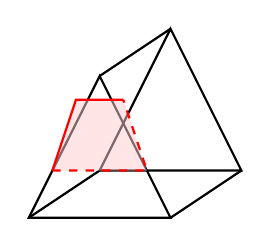
\begin{tikzpicture}[scale=0.6]
  % Front triangle
  \draw[thick] (0,0) -- (3,0) -- (1.5,3) -- cycle;
  % Back triangle
  \draw[thick] (1.5,1) -- (4.5,1) -- (3,4) -- cycle;
  % Connecting edges
  \draw[thick] (0,0) -- (1.5,1);
  \draw[thick] (3,0) -- (4.5,1);
  \draw[thick] (1.5,3) -- (3,4);
  % Cross section
  \fill[red!20,opacity=0.5] (0.5,1) -- (2.5,1) -- (2,2.5) -- (1,2.5) -- cycle;
  \draw[thick,red,dashed] (0.5,1) -- (2.5,1) -- (2,2.5);
  \draw[thick,red] (0.5,1) -- (1,2.5) -- (2,2.5);
\end{tikzpicture}
\end{center}
\end{questionText}
\choiceA{Rectangle}
\choiceB{Triangle}
\choiceC{Circle}
\choiceD{Hexagon}
\correctAnswer{B}
\explanation{A cut parallel to the base of a prism gives a shape congruent to the base. Since the base is a triangle, the cross-section is a triangle.}
\end{practiceQuestion}

\begin{practiceQuestion}{7-3-q29}{gsa}
\begin{questionText}
The diagram shows a circular swimming pool. Find the area of the pool. Use $\pi \approx 3.14$.

\begin{center}
\begin{tikzpicture}[scale=0.4]
  \fill[cyan!20] (0,0) circle (3.5);
  \draw[thick,funBlue] (0,0) circle (3.5);
  \fill (0,0) circle (2pt) node[below] {center};
  \draw[thick,funRed,<->] (-3.5,0) -- (3.5,0);
  \node[above,funRed] at (0,0.2) {$18$ m};
\end{tikzpicture}
\end{center}
\end{questionText}
\correctAnswer{$254.34$ m$^2$}
\explanation{$r = 18 \div 2 = 9$ m. $A = \pi r^2 = 3.14 \times 81 = 254.34$ m$^2$.}
\end{practiceQuestion}

\begin{practiceQuestion}{7-4-q12}{mc}
\begin{questionText}
A square has sides of $10$ m. A quarter circle with radius $10$ m is removed from one corner. What is the area of the remaining figure? Use $\pi \approx 3.14$.
\end{questionText}
\choiceA{$21.5$ m$^2$}
\choiceB{$50$ m$^2$}
\choiceC{$78.5$ m$^2$}
\choiceD{$100$ m$^2$}
\correctAnswer{A}
\explanation{Square: $100$ m$^2$. Quarter circle: $\frac{1}{4} \times 3.14 \times 100 = 78.5$ m$^2$. Remaining: $100 - 78.5 = 21.5$ m$^2$.}
\end{practiceQuestion}

\begin{practiceQuestion}{7-5-q28}{gmc}
\begin{questionText}
The diagram shows a triangular prism. What is its total surface area?

\begin{center}
\begin{tikzpicture}[scale=0.4]
  % Front triangle
  \draw[thick,funBlue,fill=funBlue!10] (0,0) -- (6,0) -- (3,4) -- cycle;
  % Back triangle (offset)
  \draw[thick,funBlue,fill=funBlue!20] (2,1.5) -- (8,1.5) -- (5,5.5) -- cycle;
  % Connecting edges
  \draw[thick,funBlue] (0,0) -- (2,1.5);
  \draw[thick,funBlue] (6,0) -- (8,1.5);
  \draw[thick,funBlue] (3,4) -- (5,5.5);
  % Labels
  \node[below] at (3,0) {$6$ cm};
  \node[left] at (1.2,2) {$5$ cm};
  \node[right] at (4.8,2) {$5$ cm};
  \node[right] at (8,3.5) {$8$ cm};
  \node[above left] at (1,0.8) {$h = 4$ cm};
\end{tikzpicture}
\end{center}
\end{questionText}
\choiceA{$104$ cm$^2$}
\choiceB{$128$ cm$^2$}
\choiceC{$152$ cm$^2$}
\choiceD{$160$ cm$^2$}
\correctAnswer{C}
\explanation{Two triangles: $2 \times \frac{1}{2} \times 6 \times 4 = 24$ cm$^2$. Three rectangles: $6 \times 8 + 5 \times 8 + 5 \times 8 = 48 + 40 + 40 = 128$ cm$^2$. Total: $24 + 128 = 152$ cm$^2$.}
\end{practiceQuestion}

\begin{practiceQuestion}{7-6-q13}{mc}
\begin{questionText}
If you triple the height of a rectangular prism while keeping the base the same, what happens to the volume?
\end{questionText}
\choiceA{It stays the same}
\choiceB{It doubles}
\choiceC{It triples}
\choiceD{It increases by a factor of $9$}
\correctAnswer{C}
\explanation{$V = Bh$. If $h$ becomes $3h$, then $V = B(3h) = 3Bh$. The volume triples.}
\end{practiceQuestion}

\begin{practiceQuestion}{8-1-q10}{mc}
\begin{questionText}
Which question would require sampling rather than surveying the entire population?
\end{questionText}
\choiceA{How many students are in a classroom of $25$?}
\choiceB{What is the average lifespan of a light bulb produced by a factory?}
\choiceC{What is the total number of books on a shelf?}
\choiceD{How many chairs are in a room?}
\correctAnswer{B}
\explanation{Testing every light bulb would destroy them all. Sampling lets you estimate the average without testing every one.}
\end{practiceQuestion}

\begin{practiceQuestion}{8-3-q08}{mc}
\begin{questionText}
The dot plots for two classes overlap significantly. The difference in their means is $2$ points, and both have a MAD of $6$. What can you conclude?
\end{questionText}
\choiceA{The classes are very different}
\choiceB{The difference in means is meaningful}
\choiceC{The difference in means is small relative to the variability}
\choiceD{You cannot compare the classes}
\correctAnswer{C}
\explanation{The difference ($2$) is much smaller than the MAD ($6$), so the difference is not very meaningful — there is a lot of overlap.}
\end{practiceQuestion}

\begin{practiceQuestion}{8-4-q06}{mc}
\begin{questionText}
Team X: mean $82$, MAD $5$. Team Y: mean $76$, MAD $5$. Which team performed better on average, and is the difference meaningful?
\end{questionText}
\choiceA{Team X; no, because the difference is less than $2$ MADs}
\choiceB{Team X; yes, because $\frac{6}{5} = 1.2$ MADs, which is meaningful}
\choiceC{Team X; yes, because the means are more than $2$ MADs apart}
\choiceD{Team Y; yes, because its MAD is the same}
\correctAnswer{A}
\explanation{Difference $= 82 - 76 = 6$. In MADs: $\frac{6}{5} = 1.2$. Since $1.2 < 2$, the difference is not considered very meaningful.}
\end{practiceQuestion}

\begin{practiceQuestion}{8-7-q29}{gsa}
\begin{questionText}
The double bar graph compares test scores for two classes over three tests.

\begin{center}
\begin{tikzpicture}[scale=0.5]
  \draw[thick,->] (0,0) -- (0,6.5) node[above]{\small Average Score};
  \draw[thick,->] (0,0) -- (8.5,0);
  % Test 1
  \fill[funBlue!70] (0.5,0) rectangle (1.5,4);
  \fill[funOrange!70] (1.6,0) rectangle (2.6,3.5);
  \node[below,font=\tiny] at (1.55,0) {Test 1};
  % Test 2
  \fill[funBlue!70] (3.2,0) rectangle (4.2,4.5);
  \fill[funOrange!70] (4.3,0) rectangle (5.3,5);
  \node[below,font=\tiny] at (4.25,0) {Test 2};
  % Test 3
  \fill[funBlue!70] (5.9,0) rectangle (6.9,5);
  \fill[funOrange!70] (7.0,0) rectangle (8.0,4);
  \node[below,font=\tiny] at (6.95,0) {Test 3};
  \foreach \y in {1,...,6} { \draw (-0.1,\y) -- (0.1,\y); \node[left,font=\tiny] at (0,\y) {$\y\times 15$}; }
  \node[above,font=\tiny] at (1,4) {$60$};
  \node[above,font=\tiny] at (2.1,3.5) {$52$};
  \node[above,font=\tiny] at (3.7,4.5) {$68$};
  \node[above,font=\tiny] at (4.8,5) {$75$};
  \node[above,font=\tiny] at (6.4,5) {$75$};
  \node[above,font=\tiny] at (7.5,4) {$60$};
\end{tikzpicture}
\end{center}

Class A (blue): $60, 68, 75$. Class B (orange): $52, 75, 60$. Find the mean for each class. Which class improved more consistently?
\end{questionText}
\correctAnswer{Class A mean $\approx 67.7$; Class B mean $= 62.3$. Class A improved consistently (scores went up each test).}
\explanation{Class A: $\frac{60+68+75}{3} = \frac{203}{3} \approx 67.7$. Class B: $\frac{52+75+60}{3} = \frac{187}{3} \approx 62.3$. Class A's scores increased each test; Class B went up then down.}
\end{practiceQuestion}

\begin{practiceQuestion}{9-4-q13}{mc}
\begin{questionText}
A probability model has outcomes A, B, and C with $P(A) = 0.5$ and $P(B) = 0.3$. What is $P(C)$?
\end{questionText}
\choiceA{$0.8$}
\choiceB{$0.3$}
\choiceC{$0.2$}
\choiceD{$0.1$}
\correctAnswer{C}
\explanation{All probabilities must sum to $1$. $P(C) = 1 - 0.5 - 0.3 = 0.2$.}
\end{practiceQuestion}

\begin{practiceQuestion}{9-6-q09}{mc}
\begin{questionText}
A bag has $3$ red and $2$ blue marbles. You draw one marble, replace it, and draw again. What is the probability that both are red?
\end{questionText}
\choiceA{$\frac{6}{25}$}
\choiceB{$\frac{9}{25}$}
\choiceC{$\frac{3}{10}$}
\choiceD{$\frac{6}{20}$}
\correctAnswer{B}
\explanation{With replacement: $P = \frac{3}{5} \times \frac{3}{5} = \frac{9}{25}$.}
\end{practiceQuestion}

\begin{practiceQuestion}{9-7-q22}{sa}
\begin{questionText}
A simulation of $50$ coin flips produces $22$ heads. Predict how many heads you would expect in $200$ flips based on this simulation.
\end{questionText}
\correctAnswer{$88$}
\explanation{Experimental $P(\text{heads}) = \frac{22}{50} = 0.44$. In $200$ flips: $200 \times 0.44 = 88$.}
\end{practiceQuestion}
